% Result plots (no macro wrappers; avoids float/stack issues)

\begin{figure}[t]
  \centering
  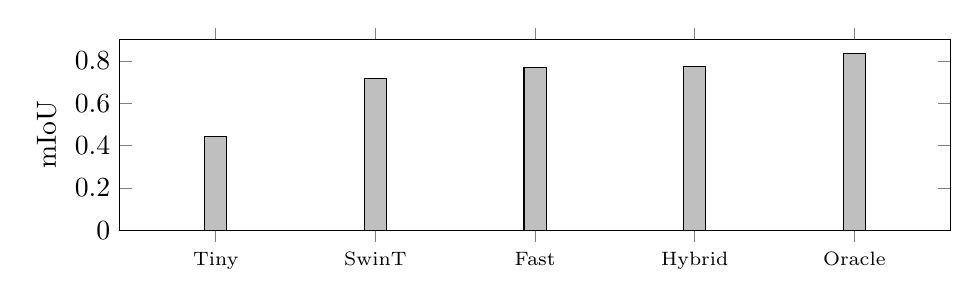
\begin{tikzpicture}
    \begin{axis}[
      width=\linewidth,
      height=4.0cm,
      ybar,
      bar width=8pt,
      ymin=0, ymax=0.90,
      ylabel={mIoU},
      symbolic x coords={Tiny,SwinT,Fast,Hybrid,Oracle},
      xtick=data,
      xticklabel style={font=\scriptsize},
      enlarge x limits=0.15,
    ]
      \addplot[fill=gray!50] coordinates {
        (Tiny,0.441) (SwinT,0.717) (Fast,0.769) (Hybrid,0.772) (Oracle,0.836)
      };
    \end{axis}
  \end{tikzpicture}
  \caption{Mask mIoU on RefCOCO val ($n{=}3{,}811$). Hybrid +5.5 mIoU over DINO-SwinT; 92.3\% of oracle.}
  \label{fig:bar-miou}
\end{figure}

\begin{figure}[t]
  \centering
  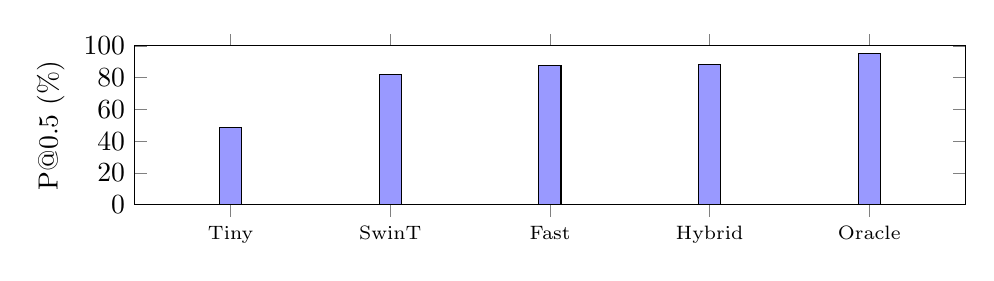
\begin{tikzpicture}
    \begin{axis}[
      width=\linewidth,
      height=3.6cm,
      ybar,
      bar width=8pt,
      ymin=0, ymax=100,
      ylabel={P@0.5 (\%)},
      symbolic x coords={Tiny,SwinT,Fast,Hybrid,Oracle},
      xtick=data,
      xticklabel style={font=\scriptsize},
      enlarge x limits=0.15,
    ]
      \addplot[fill=blue!40] coordinates {
        (Tiny,48.6) (SwinT,81.7) (Fast,87.5) (Hybrid,88.1) (Oracle,95.2)
      };
    \end{axis}
  \end{tikzpicture}
  \caption{Precision at mask IoU $\geq 0.5$ (RefCOCO val).}
  \label{fig:bar-p05}
\end{figure}

\begin{figure}[t]
  \centering
  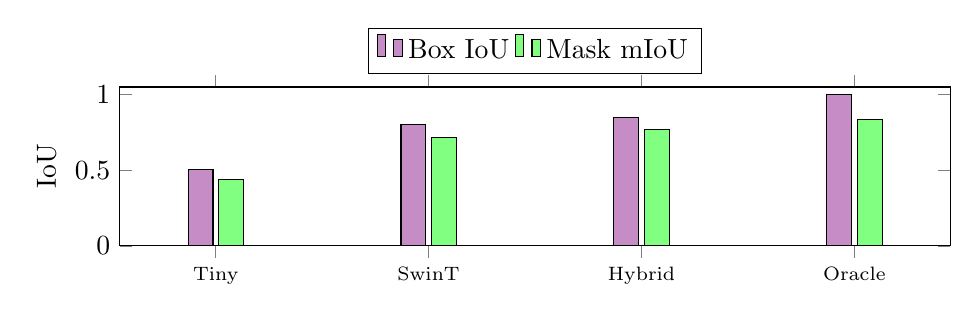
\begin{tikzpicture}
    \begin{axis}[
      width=\linewidth,
      height=3.6cm,
      ybar,
      bar width=9pt,
      ymin=0, ymax=1.05,
      ylabel={IoU},
      symbolic x coords={Tiny,SwinT,Hybrid,Oracle},
      xtick=data,
      xticklabel style={font=\scriptsize},
      legend style={at={(0.5,1.08)}, anchor=south, legend columns=2},
      enlarge x limits=0.15,
    ]
      \addplot[fill=violet!45] coordinates {(Tiny,0.506) (SwinT,0.802) (Hybrid,0.851) (Oracle,1.000)};
      \addplot[fill=green!50] coordinates {(Tiny,0.441) (SwinT,0.717) (Hybrid,0.772) (Oracle,0.836)};
      \legend{Box IoU, Mask mIoU}
    \end{axis}
  \end{tikzpicture}
  \caption{Box IoU vs.\ mask mIoU (RefCOCO val).}
  \label{fig:box-mask}
\end{figure}

\begin{figure}[t]
  \centering
  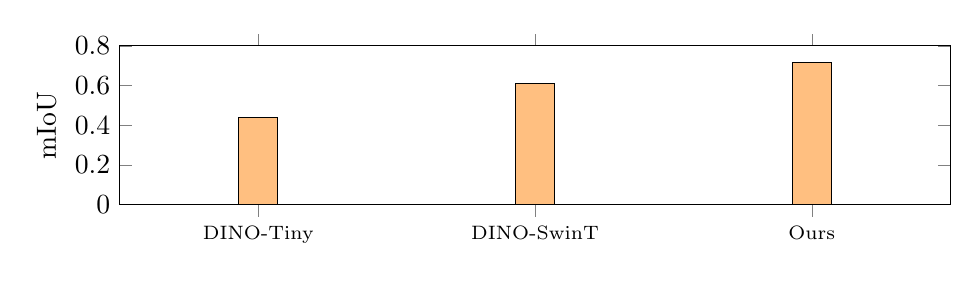
\begin{tikzpicture}
    \begin{axis}[
      width=\linewidth,
      height=3.6cm,
      ybar,
      bar width=14pt,
      ymin=0, ymax=0.80,
      ylabel={mIoU},
      symbolic x coords={Tiny,SwinT,Hybrid},
      xtick=data,
      xticklabels={DINO-Tiny,DINO-SwinT,Ours},
      xticklabel style={font=\scriptsize},
      enlarge x limits=0.25,
    ]
      \addplot[fill=orange!50] coordinates {(Tiny,0.440) (SwinT,0.612) (Hybrid,0.717)};
    \end{axis}
  \end{tikzpicture}
  \caption{RefCOCO+ val ($n{=}3{,}805$). Hybrid +10.5 mIoU over DINO-SwinT.}
  \label{fig:refcoco-plus}
\end{figure}

\begin{figure}[t]
  \centering
  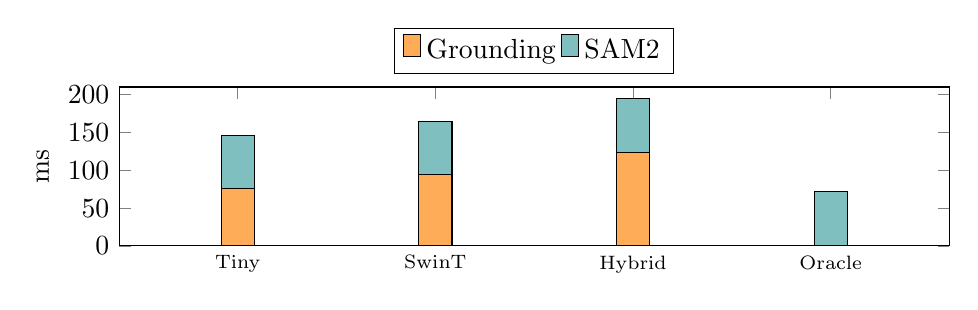
\begin{tikzpicture}
    \begin{axis}[
      width=\linewidth,
      height=3.6cm,
      ybar stacked,
      bar width=12pt,
      ymin=0, ymax=210,
      ylabel={ms},
      symbolic x coords={Tiny,SwinT,Hybrid,Oracle},
      xtick=data,
      xticklabel style={font=\scriptsize},
      legend style={at={(0.5,1.08)}, anchor=south, legend columns=2},
      enlarge x limits=0.2,
    ]
      \addplot[fill=orange!65] coordinates {(Tiny,76) (SwinT,94) (Hybrid,124) (Oracle,0)};
      \addplot[fill=teal!50] coordinates {(Tiny,70) (SwinT,71) (Hybrid,71) (Oracle,72)};
      \legend{Grounding, SAM2}
    \end{axis}
  \end{tikzpicture}
  \caption{Mean latency (RefCOCO val): 146 / 164 / 195 / 72\,ms total.}
  \label{fig:latency}
\end{figure}

\begin{figure}[t]
  \centering
  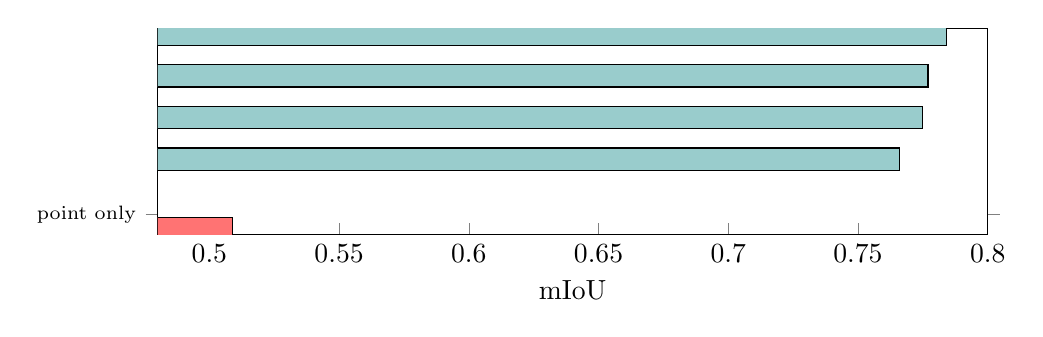
\begin{tikzpicture}
    \begin{axis}[
      width=\linewidth,
      height=4.2cm,
      xbar,
      bar width=8pt,
      xmin=0.48, xmax=0.80,
      xlabel={mIoU},
      symbolic y coords={point,boxpt,top1,default,full},
      yticklabels={point only, box+point, top1, default, no crop},
      ytick=data,
      yticklabel style={font=\scriptsize},
      enlarge y limits=0.12,
    ]
      \addplot[fill=red!55] coordinates {(0.509,point)};
      \addplot[fill=teal!40] coordinates {(0.766,boxpt) (0.775,top1) (0.777,default) (0.784,full)};
    \end{axis}
  \end{tikzpicture}
  \caption{Adapter ablations (200-ref subset).}
  \label{fig:ablation-bar}
\end{figure}
